\documentclass{article}

\usepackage{graphicx}
\PassOptionsToPackage{hyphens}{url}\usepackage[hidelinks]{hyperref}
\usepackage{listings}
\usepackage{float}

\title{
	\huge Hemp Tracker\\
	\normalsize Trazabilidad de cáñamo basado en tecnología blockchain.
}
\author{
	Gallardo, Esmeralda\\
	\texttt{esmeralda.gallardo@fing.edu.uy}\\
	Rodríguez, Guillermo\\
	\texttt{guillermor@fing.edu.uy}\\
	Rodríguez, Viterbo\\
	\texttt{viterbo.rodriguez@fing.edu.uy}
}
\date{2021-01-04}

\begin{document}

\makeatletter
\begin{titlepage}
	\begin{center}
		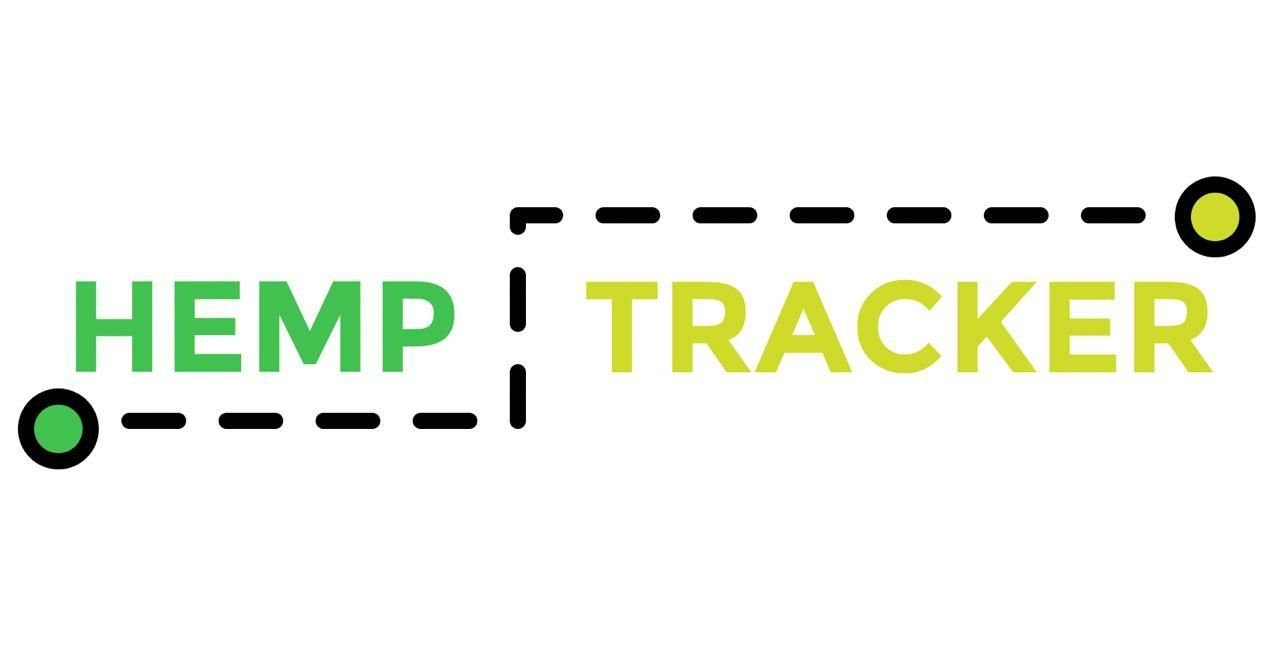
\includegraphics[width=\linewidth]{res/logotype.jpg}\\
		{\large \bfseries Trazabilidad de cáñamo basado en tecnología blockchain.}\\[1in]
		\@author\\[1in]
		{\large \@date}
	\end{center}
\end{titlepage}
\makeatother
\thispagestyle{empty}

\newpage

All rights reserved.

Todos los derechos reservados.

\textcopyright

2021
\newpage
\pagenumbering{gobble}
\tableofcontents
\newpage
\pagenumbering{arabic}
\setcounter{page}{1}
\section{Introducción}
La industria del cáñamo está empezando a ganar terreno en un mundo que ya empieza a tener los primeros países pioneros en regular y despenalizar el uso recreativo y/o medicinal de las plantas. La propuesta de Hemp Tracker es servir a los productores a mejorar la transparencia de todo el proceso de producción de cáñamo y llevar toda esa información al consumidor final desde el mismo envase del producto.

Hemp Tracker es la diferencia entre comprar un producto de procedencia dudosa o totalmente desconocida, a tener toda la información al instante en tu celular. Los productores que se sirvan de esta solución para trazar su producción y competir en transparencia contarán con una clara ventaja en el mercado.
\newpage

\section{HempTracker MVP}

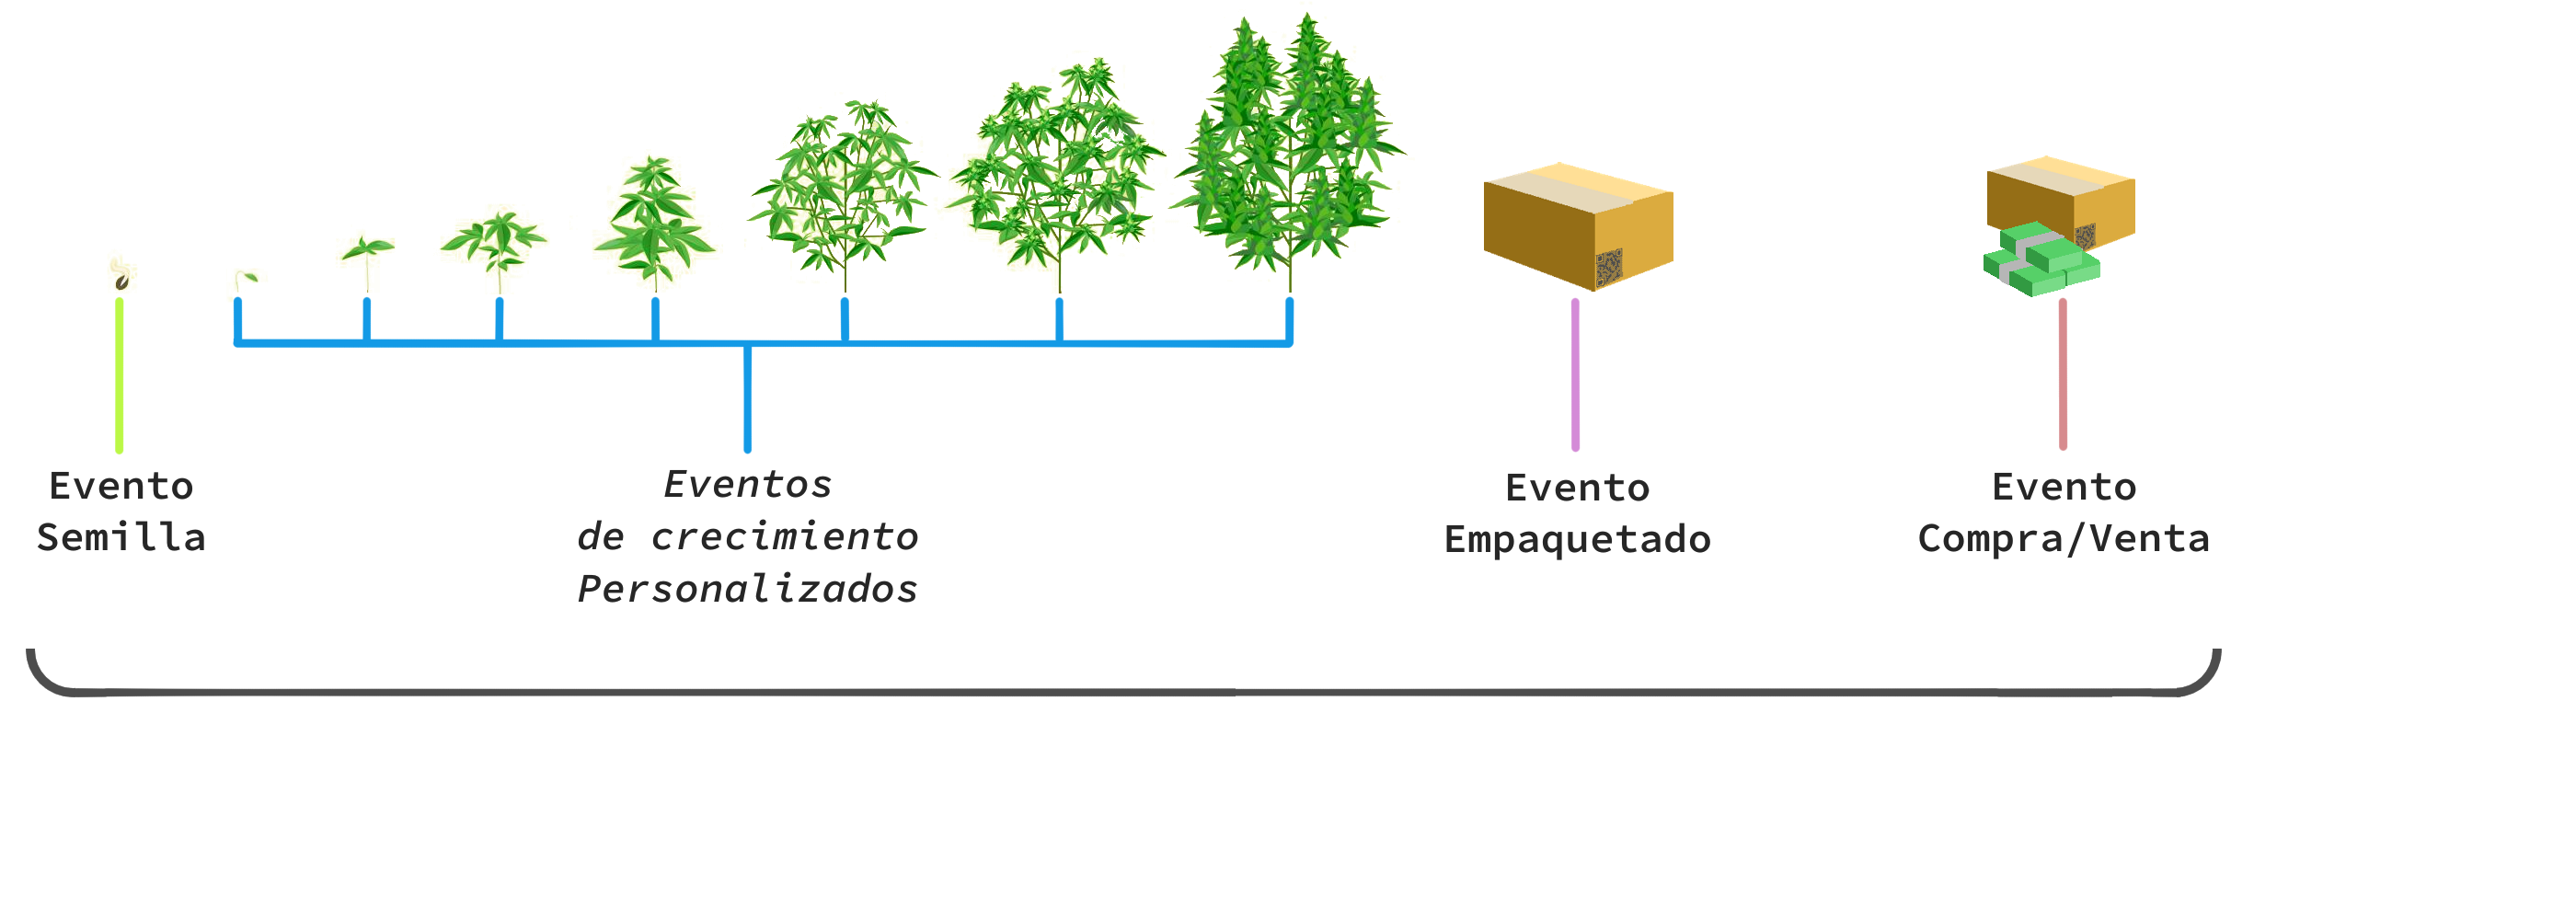
\includegraphics[width=\linewidth]{res/events.png}

Se propone un sistema multi-usuario donde dependiendo del rol se brinda una interfaz web personalizada para poder registrar en la blockchain cada paso de la cadena de producción.

Si bien contamos con un modelo de producción estándar extraído de experiencias de productores locales, una de las grandes ventajas de nuestro sistema es su adaptabilidad permitiendo así brindar una solución a medida.

Nuestro modelo estándar contempla los siguientes roles:

\begin{itemize}
	\item \textit{Agrimensor}
	\subitem Registra zonas de cultivo de un \textit{Productor}.
	\item \textit{Meteorólogo}
	\subitem Ingresa eventos meteorológicos en una zona.
	\item \textit{Certificador}
	\subitem Ente que emite certificados, sobre métodos de producción o orgánicos, pueden ser entes estatales o privados.
	\item \textit{Productor de semilla}
	\subitem Produce y vende semillas de cáñamo.
	\item \textit{Vivero}
	\subitem Vende servicios de germinacion.
	\item \textit{Productor}
	\subitem Planta semillas, puede registrar eventos de crecimiento, podas, curas, y muchos mas, culminando en la cosecha de flores.
	\item \textit{Broker}
	\subitem Comerciante mayorista.
\end{itemize}

\subsection{Estructura}

\subsection{Servicios}

\begin{itemize}
	\item \textit{visitante}: puede ojear en "las páginas" de información que tenemos, indexadas por varios criterios y todo de forma anónima.
	\item \textit{productor}: además de ser visitante, puede registrarse y solicitar el rol de "producer". Una vez que lo obtenga puede loguearse, acceder a un perfil y acceder a sus plantaciones donde podrá dar de alta nuevas plantaciones y administrar sus datos (nombres, fechas, números).
	\item \textit{admin}: nosotros podremos dar de alta la organización "hemptracker.net", podremos dar de alta los roles ("producer", "admin", etc), aceptar o rechazar Requests de asignación de roles. 
	\item \textit{rolX}: podrá registrar "eventos" sobre una plantación concreta. Pudiendo además especificar si es sobre toda la plantación, una porción o un grupo concreto. Se registra el account, el profile, el rol, la fecha, y una string con un json describiendo el evento.
\end{itemize}


\newpage

\begin{thebibliography}{120}

	\bibitem{item_id} Item text

\end{thebibliography}

\newpage

\section{Apendice: Normativa internacional}

A continuación una investigación sobre las diversas certificaciones de la industria del cáñamo en algunos países de interés:

\begin{itemize}
	\item Uruguay
	\item Suiza
	\item Unión Europea
	\item Canadá
	\item Estados Unidos
\end{itemize}

\newpage

\subsection{Uruguay}

\subsubsection{Ley 19.172 - Decreto reglamentario 372/14}

\begin{itemize}
	\item Definición: Cáñamo Industrial
	\subitem Planta, órganos y derivados con un contenido de THC \textless 1\%
	\subitem Semillas con un contenido THC \textless 0,5\%
	\item Actividades (Autorizaciones por el MGAP)
	\subitem Importación y Exportación
	\subitem Plantación, Cultivo, Cosecha y Comercialización
	\subitem Industrialización: Volúmenes y condiciones
\end{itemize}

\subsubsection{Decreto reglamentario 46/15}
Autorizaciones del IRCCA y MSP. Según uso del Cannabis psicoactivo y no psicoactivo.

\begin{itemize}
	\item Medicinal
	\subitem Especialidades Vegetales: hierba y/o mezclas
	\subitem Especialidades Farmacéuticas: Medicamento a base de Cannabis
	\item Científico
	\subitem Proyectos de investigación científica
\end{itemize}

\subsubsection{Organismos}

\begin{itemize}
	\item MGAP - Ministerio de Ganadería Agricultura y Pesca
	\subitem \url{www.gub.uy/ministerio-ganaderia-agricultura-pesca}
	\item MSP - Ministerio de Salud Publica
	\subitem \url{www.gub.uy/ministerio-salud-publica}
	\item INASE - Instituto Nacional de Semillas
	\subitem \url{www.inase.uy}
	\item IRCCA - Instituto de Regulación y Control del Cannabis
	\subitem \url{www.ircca.gub.uy}
	\item SENACLAFT - Secretaría Nacional para la Lucha contra el Lavado de Activos y el Financiamiento del Terrorismo
	\subitem \url{www.gub.uy/secretaria-nacional-lucha-contra-lavado-activos-financiamiento-terrorismo/}
\end{itemize}

\subsubsection{Noticias}

\begin{itemize}
	
	\item GlobalNewsWire - ICC LABS Inc. - 11 de mayo de 2018
	\subitem \url{www.globenewswire.com/news-release/2018/05/11/1501065/0/en/ICC-Labs-Receives-Organic-Hemp-Certification-Readies-for-Harvest-and-Continues-Construction-of-Laboratory.html}
	\subitem "Alejandro Antalich, added, “Our first outdoor harvest will give our technicians the opportunity to discover the behavior of the three different strains that we have cultivated. In Uruguay, we are growing and producing according to high quality standards, such as Good Agricultural Practices (GAP) and, with respect to the Canelones site, our newly obtained organic certification. Further, construction of our 33,175 sq. ft. CO2 CBD extraction laboratory in accordance with Good Manufacturing Practices (GMP) is proceeding and we estimate that it is almost 90\% complete.”"
	
	\item El Observador - Exportadora CPLANT - 10 de agosto de 2020
	\subitem \url{www.elobservador.com.uy/nota/empresa-uruguaya-eleva-la-exportacion-de-flores-de-canamo-14-toneladas-en-dos-meses-202081013239}
	\subitem "La empresa posee la certificación GACP (Good agricultural and collection practices) validada en Europa y por la Organización Mundial de la Salud (OMS) y cumple en todos sus procesos las normativas GMP (Good manufacturing practices)."
\end{itemize}

\subsubsection{Otros links}

\url{www.gub.uy/ministerio-ganaderia-agricultura-pesca/tramites-y-servicios/servicios/licencia-autorizacion-operacion-canamo}

\newpage

\subsection{Suiza}

\subsubsection{Normativa}

El cannabis que contiene más del 1,0\% de THC está clasificado como droga ilegal en Suiza. Así, de acuerdo con la Ley Federal de Drogas: la producción, cultura, uso y posesión de cannabis están prohibidos y considerados como infracciones penales. Estas infracciones se castigan con hasta tres años de prisión y / o multa.

Desde 2017, el cannabis legal, también conocido como "hierba baja en THC", con menos del 1,0\% de THC se vende en casi todas las tiendas de tabaco. En marzo de 2019, un Tribunal Administrativo Federal suizo confirmó el esquema de impuestos de los funcionarios de aduanas, que imponen un impuesto de CHF38 (\$ 37.70) por kilo, así como el 25\% de los ingresos minoristas.

\subsubsection{IG Hemp}

\centerline{"For a strong hemp market in Switzerland"}

"Interest Group Hemp es la asociación de productores y comerciantes de cáñamo suizos. Promovemos el intercambio y cooperación entre miembros y para fortalecer la industria del cáñamo en Suiza." 

\url{ighanf.ch/?lang=en}

\subsubsection{Swiss Certified Cannabis – SCC}
"The introduction and maintenance of a quality standard in the Swiss cannabis industry protects producers and consumers. Therefore the \textit{IG Hemp has created the quality label Swiss Certified Cannabis (SCC), which is awarded by qualified auditors.} It thus guarantees product and consumer safety. SCC sets the stage for further professionalization of the industry and strengthens cooperation with authorities and control bodies. The SCC guidelines are constantly and sensibly developed with the aim of improving the quality of cannabis products in Switzerland in the long term."

"IG Hemp creo el sello de calidad Swiss Certified Cannabis (SCC), que es otorgado por auditores calificados."

\begin{figure}[H]
	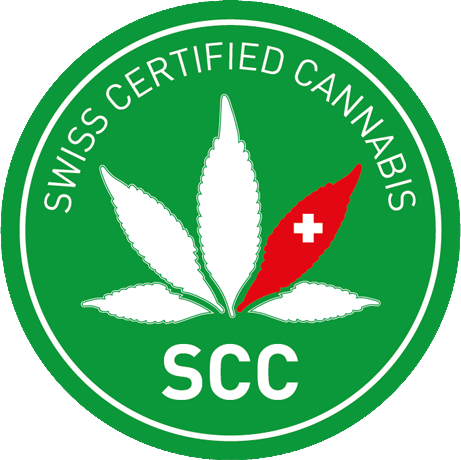
\includegraphics[width=100px]{res/su-scc.png}
	\label{fig:suscc}
\end{figure}

\url{ighanf.ch/projekte/swiss-certified-cannabis-scc/?lang=en}

\subsubsection{Bio Suisse}

\begin{itemize}
	\item Bio Suisse, a private-sector organization, is the federation of Swiss organic farmers
	\item This umbrella organization counts 32 organic farmers' associations among its members, as well as the Research Institute of Organic Agriculture FiBL.
	\item Common and uniform standards for agriculture and processing.
	\item Common label, the "Bud" (German: Knospe); organic products carrying the Bud label has a market share in Switzerland of about 10.3%
	\item More than 1'050 processing and trade companies have a licence contract with Bio Suisse to use the label
\end{itemize}

\begin{figure}[H]
	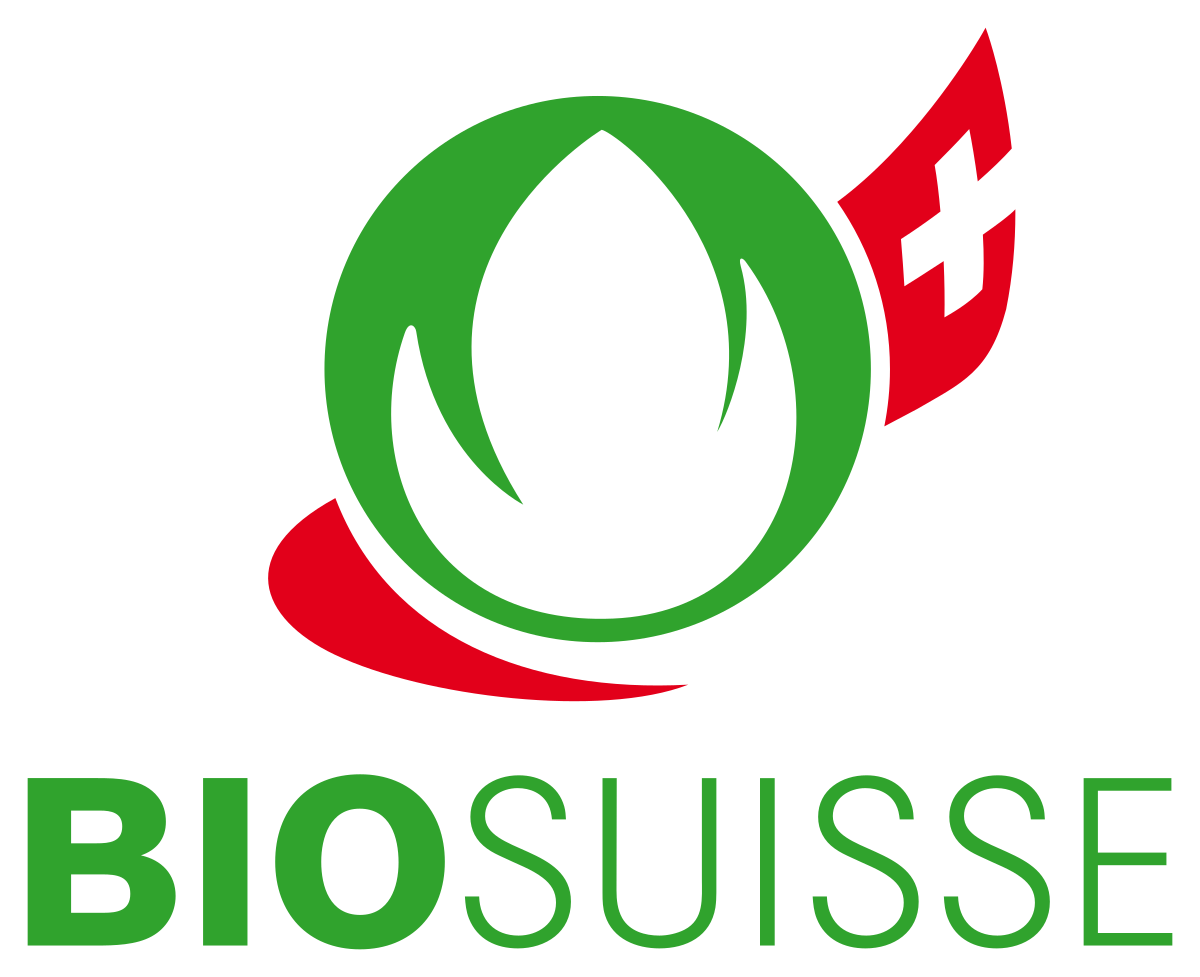
\includegraphics[width=100px]{res/su-biosuisse.png}
	\label{fig:subio}
\end{figure}

\url{www.bio-suisse.ch/en/whoisbiosuisse.php}

\newpage

\subsection{Union Europea}

\subsubsection{Normativa}

El mercado de flores de CBD en Europa gira principalmente en torno al cáñamo. Según la legislación de la UE, el cáñamo se clasifica como cannabis con menos del 0,2\% de THC en peso seco. Legalmente también debe ser de la variedad de semillas que apruebe la Unión Europea. Se puede cultivar cáñamo aprobado bajo licencia en la mayor parte de Europa. En las pruebas de laboratorio, debe contener menos del 0,2\% de THC o lo destruirán.

Además, algunos países tienen límites de THC más altos, sobre todo Suiza (1\%), Italia (.6\%) y Austria (.3\%). En algunos lugares, en una oferta para cumplir con la ley, la flor de cáñamo a menudo se abre paso como té, o solo como producto "no apto para consumo".

\subsubsection{European Industrial Hemp Association}

Tomado de su pagina web (\url{eiha.org}):

La única organización pan-europea en el sector de cáñamo industrial. Representamos los intereses tanto  de empresas productoras como procesadoras. La AIEC fue formada casi hace 19 años y oficialmente fundada en 2005, con oficinas tanto en Bruselas y Colonia.

Nuestra membresía abarca 25 estados de la UE y 12 países adicionales, incluidos miembros en América del Norte y APAC, que comprenden una membresía total de más de 200, principalmente agricultores, procesadores y fabricantes; representando toda la cadena desde la semilla hasta el estante.

\subsubsection{GMP: Good Manufacturing Practice}

\begin{figure}[H]
	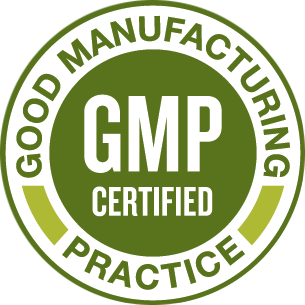
\includegraphics[width=100px]{res/eu-gmp.png}
	\label{fig:eugmp}
\end{figure}

GMP, que significa buenas prácticas de fabricación, es un sistema para garantizar que los productos se produzcan y controlen de manera constante. La Unión Europea ha armonizado su legislación con las recomendaciones de la Organización Mundial de la Salud. La certificación GMP es necesaria para comerciar con empresas farmacéuticas.

\url{www.ema.europa.eu/en/human-regulatory/research-development/compliance/good-manufacturing-practice}

\subsubsection{Certificación Orgánica}

\begin{figure}[H]
	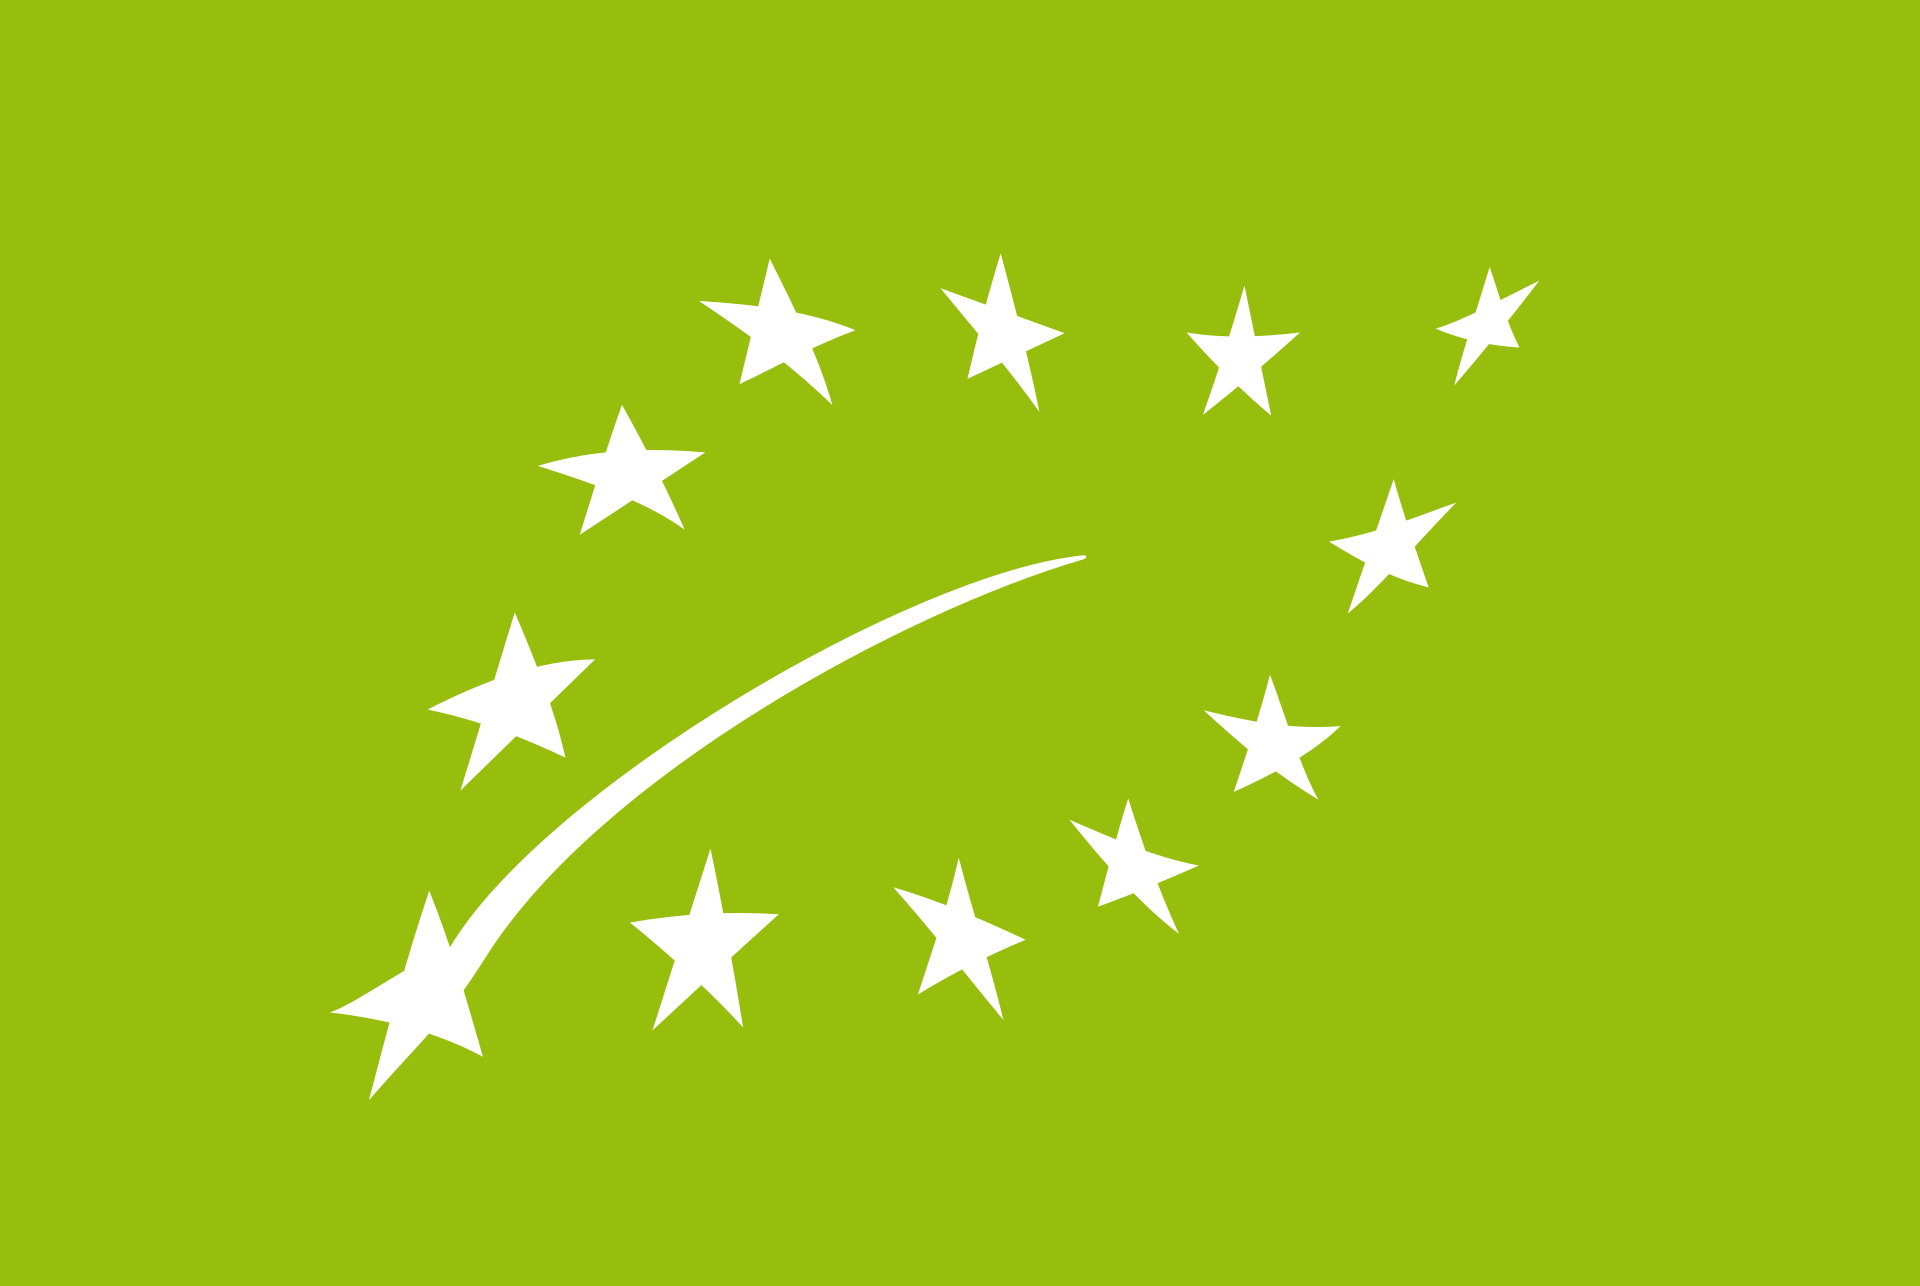
\includegraphics[width=100px]{res/eu-organic.png}
	\label{fig:euorganic}
\end{figure}

La Unión Europea también ha especificado las prácticas requeridas para la agricultura orgánica. Los productos que cumplen con estas prácticas pueden ser reconocidos por el logotipo "orgánico certificado por la UE".

\url{eur-lex.europa.eu/LexUriServ/LexUriServ.do?uri=OJ:L:2007:189:0001:0023:EN:PDF}

\newpage

\subsection{Canadá}

\subsubsection{Normativa}

El cáñamo industrial es un cannabis que contiene un 0,3 \% de THC, no hay límite en la cantidad de CBD.

Health Canada supervisa la producción de productos de cannabis. Health Canada también es responsable de supervisar la distribución y venta de cannabis, incluido cualquier producto de cannabis que contenga CBD para fines médicos.

Las provincias y territorios son responsables de determinar cómo se distribuye y vende el cannabis dentro de sus jurisdicciones.

Las Regulaciones del cáñamo industrial autorizan la importación y exportación de semillas o granos, pero no las flores, ramas u hojas, estos solo pueden ser importados o exportados por un titular de licencia en virtud de las Regulaciones sobre el cannabis:

\begin{itemize}
	\item con un permiso emitido bajo esas regulaciones
	\item para fines médicos y científicos legítimos
\end{itemize}

Para importar o exportar semillas o granos de cáñamo industrial, debe:

\begin{itemize}
	\item tener una licencia de Health Canada
	\item tener un permiso de importación o exportación emitido por Health Canada
\end{itemize}

\subsubsection{Industrial Hemp licensing application}

Este documento proporciona orientación a cualquier persona que desee solicitar una licencia ("el solicitante") en virtud de la Ley del Cannabis para realizar las siguientes actividades en relación con el cáñamo industrial:

\begin{itemize}
	\item cultivo
	\item rebaja
	\item importación
	\item exportación
	\item limpieza
	\item preparar (acondicionamiento)
	\item procesamiento (incluida la transformación en no viables y la producción de derivados / productos)
\end{itemize}

\url{www.canada.ca/en/health-canada/services/publications/drugs-health-products/industrial-hemp-licensing-application-guide.html}

\subsubsection{Certificación Orgánica}

El Régimen Orgánico de Canadá (COR) requiere la certificación obligatoria de los Estándares Orgánicos Canadienses

La CFIA regula el uso del logotipo orgánico de Canadá a continuación. El uso del logo orgánico solo está permitido en productos que tienen un contenido orgánico mayor o igual al 95\% y han sido certificados de acuerdo con los requisitos del Régimen Orgánico de Canadá. El uso del logotipo orgánico es voluntario, pero cuando se usa está sujeto a los requisitos del SFCR.

Los productos importados deben cumplir con los requisitos del Régimen Orgánico de Canadá. Los productos importados que llevan el logo deben incluir:

\begin{itemize}
	\item la declaración "Producto de", inmediatamente antes del nombre del país de origen, o
	\item la declaración "Importado", muy cerca del logotipo
\end{itemize}

Estas declaraciones deben aparecer en la etiqueta tanto en francés como en inglés, a menos que se aplique una exención de etiquetado bilingüe

\begin{figure}[H]
	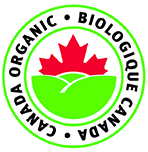
\includegraphics[width=100px]{res/ca-organic.jpg}
	\label{fig:caorgnic}
\end{figure}

\url{canada-organic.ca/en/what-we-do/organic-101/organic-certification}

\newpage

\subsection{Estados Unidos}

\subsubsection{Normativa}

El Servicio de Inspección de Sanidad Animal y Vegetal del USDA (United States Department of Agriculture) regula la importación de todas las plantas y semillas para plantar a fin de garantizar un comercio agrícola seguro.

El término "cáñamo" significa la planta Cannabis sativa L. y cualquier parte de esa planta, incluidas sus semillas y todos los derivados, extractos, cannabinoides, isómeros, ácidos, sales y sales de isómeros, ya sea en crecimiento o no, con un delta. -9 concentración de tetrahidrocannabinol(THC) no superior al 0,3 \% en peso seco.

Las plantas de cáñamo se pueden importar a los Estados Unidos desde países distintos a Canadá si van acompañadas de ambos:

\begin{enumerate}
	\item Un certificado fitosanitario de la ONPF del país exportador para verificar el origen de la planta y confirmar que no se detectan plagas de plantas; y
	\item Un permiso PPQ 587, Solicitud de permiso para importar plantas o productos vegetales.
\end{enumerate}
\url{www.aphis.usda.gov/library/forms/pdf/PPQ587.pdf}\\
\url{www.aphis.usda.gov/aphis/ourfocus/planthealth/import-information/hemp}

\subsubsection{Certificación Orgánica}

El Programa Orgánico Nacional (NOP) desarrolla las reglas y regulaciones para la producción, manejo, etiquetado y cumplimiento de todos los productos orgánicos del USDA. Este proceso, al que se hace referencia como elaboración de normas, implica aportaciones de la Junta Nacional de Normas Orgánicas (un Comité Asesor Federal formado por quince miembros del público) y del público. El NOP también mantiene un Manual que incluye orientación, instrucciones, memorandos de políticas y otros documentos que comunican los estándares orgánicos.

\begin{figure}[H]
	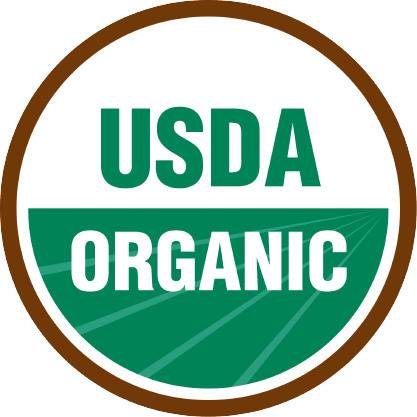
\includegraphics[width=100px]{res/usa-organic.png}
	\label{fig:usaorgnic}
\end{figure}

\url{www.usda.gov/topics/organic}

\url{www.ams.usda.gov/rules-regulations/organic}

\url{www.ams.usda.gov/services/organic-certification/becoming-certified}

\end{document}